\section{Experiments}
The data come from the MNIST dataset, containing 60000 train images and 10000 test images from 10 almost balanced classes (arabic numerals). The following simulations generate a universal adversarial perturbation starting from a portion of the MNIST test dataset. Then the perturbation is added to the test images that have been correctly classified by the pre-trained LeNet-5 convolutional neural network, aiming to maximally increase the loss function, and therefore minimize the accuracy.\\
In particular, the perturbation has to inject a minimal visual distortion to the original images and this is ensured by the constraint on the $\ell_{\infty}$ norm in the optimization problem (1). Therefore, the digits in the perturbed images still appear clearly distinguishable to the human eyes, but get misclassified by LeNet5.\\
In the following experiments, the $\ell_{\infty}$ norm of the perturbation is chosen so as not to be higher than $\varepsilon=0.25$.\\

For semplicity, all the algorithms introduced in the previous section have been implemented in a sequential fashion, rather than using a proper distributed architecture. Therefore, the workers do not effectly represent different processors in different machines, but they are just different methods called by the same machine, imitating a distributed setting. Nevertheless, all the algorithms can be easily modified to accomodate a proper distributed architecture by configuring Ray\footnote{Ray: https://github.com/ray-project/ray.} or PySpark\footnote{PySpark: https://spark.apache.org/docs/latest/api/python.}.\\

Again, for semplicity, the algorithms do not involve a normalization technique for the perturbed images and therefore normalization has been applied only after the computation of the universal adversarial perturbation, that is just before the testing of LeNet5. A possible improvement could be to consider the Box constraint described in \cite{A1}, section V.B.\\

In addition, a key concept of the Frank-Wolfe theory is the duality gap, that is an upper bound for the primal suboptimality $F(\mathbf{x}_t)-F(\mathbf{x}^*)$ defined as:
\begin{equation}
	\mathcal{G}(\mathbf{x}) =\max_{\mathbf{s}\in\mathit{C}} \langle \nabla F(\mathbf{x}),\mathbf{x}-\mathbf{s}\rangle.
\end{equation}
Therefore, a further improvement of the implementation could be the use of the Frank-Wolfe duality gap as stopping criterion for the algorithms. However, this turned out to be difficult in the distributed settings at hand.

\begin{figure}%[htbp]
	\centering
	\begin{subfigure}[b]{0.15\textwidth}
		\centering
		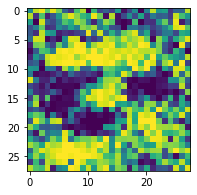
\includegraphics[width=2.5cm]{T20_final.png}
		\caption{}
		\label{fig:decentralized_perturbation}
	\end{subfigure}
	\hfill
	\begin{subfigure}[b]{0.15\textwidth}
		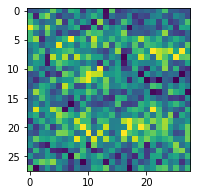
\includegraphics[width=2.5cm]{q5_n10_final.png}
		\caption{}
		\label{fig:variance-reduce_perturbation}
	\end{subfigure}
	\hfill
	\begin{subfigure}[b]{0.15\textwidth}
		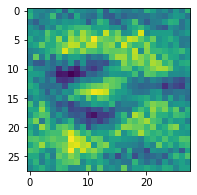
\includegraphics[width=2.5cm]{T100_final_distr.png}
		\caption{}
		\label{fig:distributed_perturbation}
	\end{subfigure}
	\caption{Perturbations of the three algorithms: \ref{fig:decentralized_perturbation} is the perturbation of the Decentralized SGF FW with T=20 and m=15, \ref{fig:variance-reduce_perturbation} is the perturbation of the Decentralized Reduced-Variance SGF FW with q=5 and n=10, \ref{fig:distributed_perturbation} is the perturbation of the Distribted SGF FW with T=100.}
	\label{fig:perturbations}
\end{figure}